\section{Resultados Experimentais}\label{sec:resultados}

Os experimentos descritos nesta seção foram realizados com o objetivo de validar o funcionamento de cada subsistema fundamental da esteira, bem como a integração entre o microcontrolador STM32G070 e o Raspberry Pi 3B. Para cada subsistema, descreve-se o procedimento adotado, os resultados obtidos e, quando pertinente, as divergências observadas e suas possíveis causas.

\paragraph{Sensores \textit{laser}.}
Os quatro sensores operam conforme especificado. A lógica de detecção síncrona por ausência de portadora foi validada com sucesso --- ao interromper o feixe, as \textit{flags} internas (\texttt{SENS1\_flag} a \texttt{SENS4\_flag}) são acionadas corretamente, permitindo as transições de estado da FSM. A mudança das flags pode ser observada na Figura ~\ref{fig:sensor_telemetry}, na seção de software. Além disso, os testes de hardware (Figura ~\ref{fig:circ_laser}) mostram que os sensores funcionaram bem em testes de bancada, como ilustrado nas figuras ~\ref{fig:laser_sem_interrupção} e ~\ref{fig:laser_interrompido}, que mostram a transição do sinal entre laser sem interromper e interrompido.

\begin{figure}[H]
    \centering
    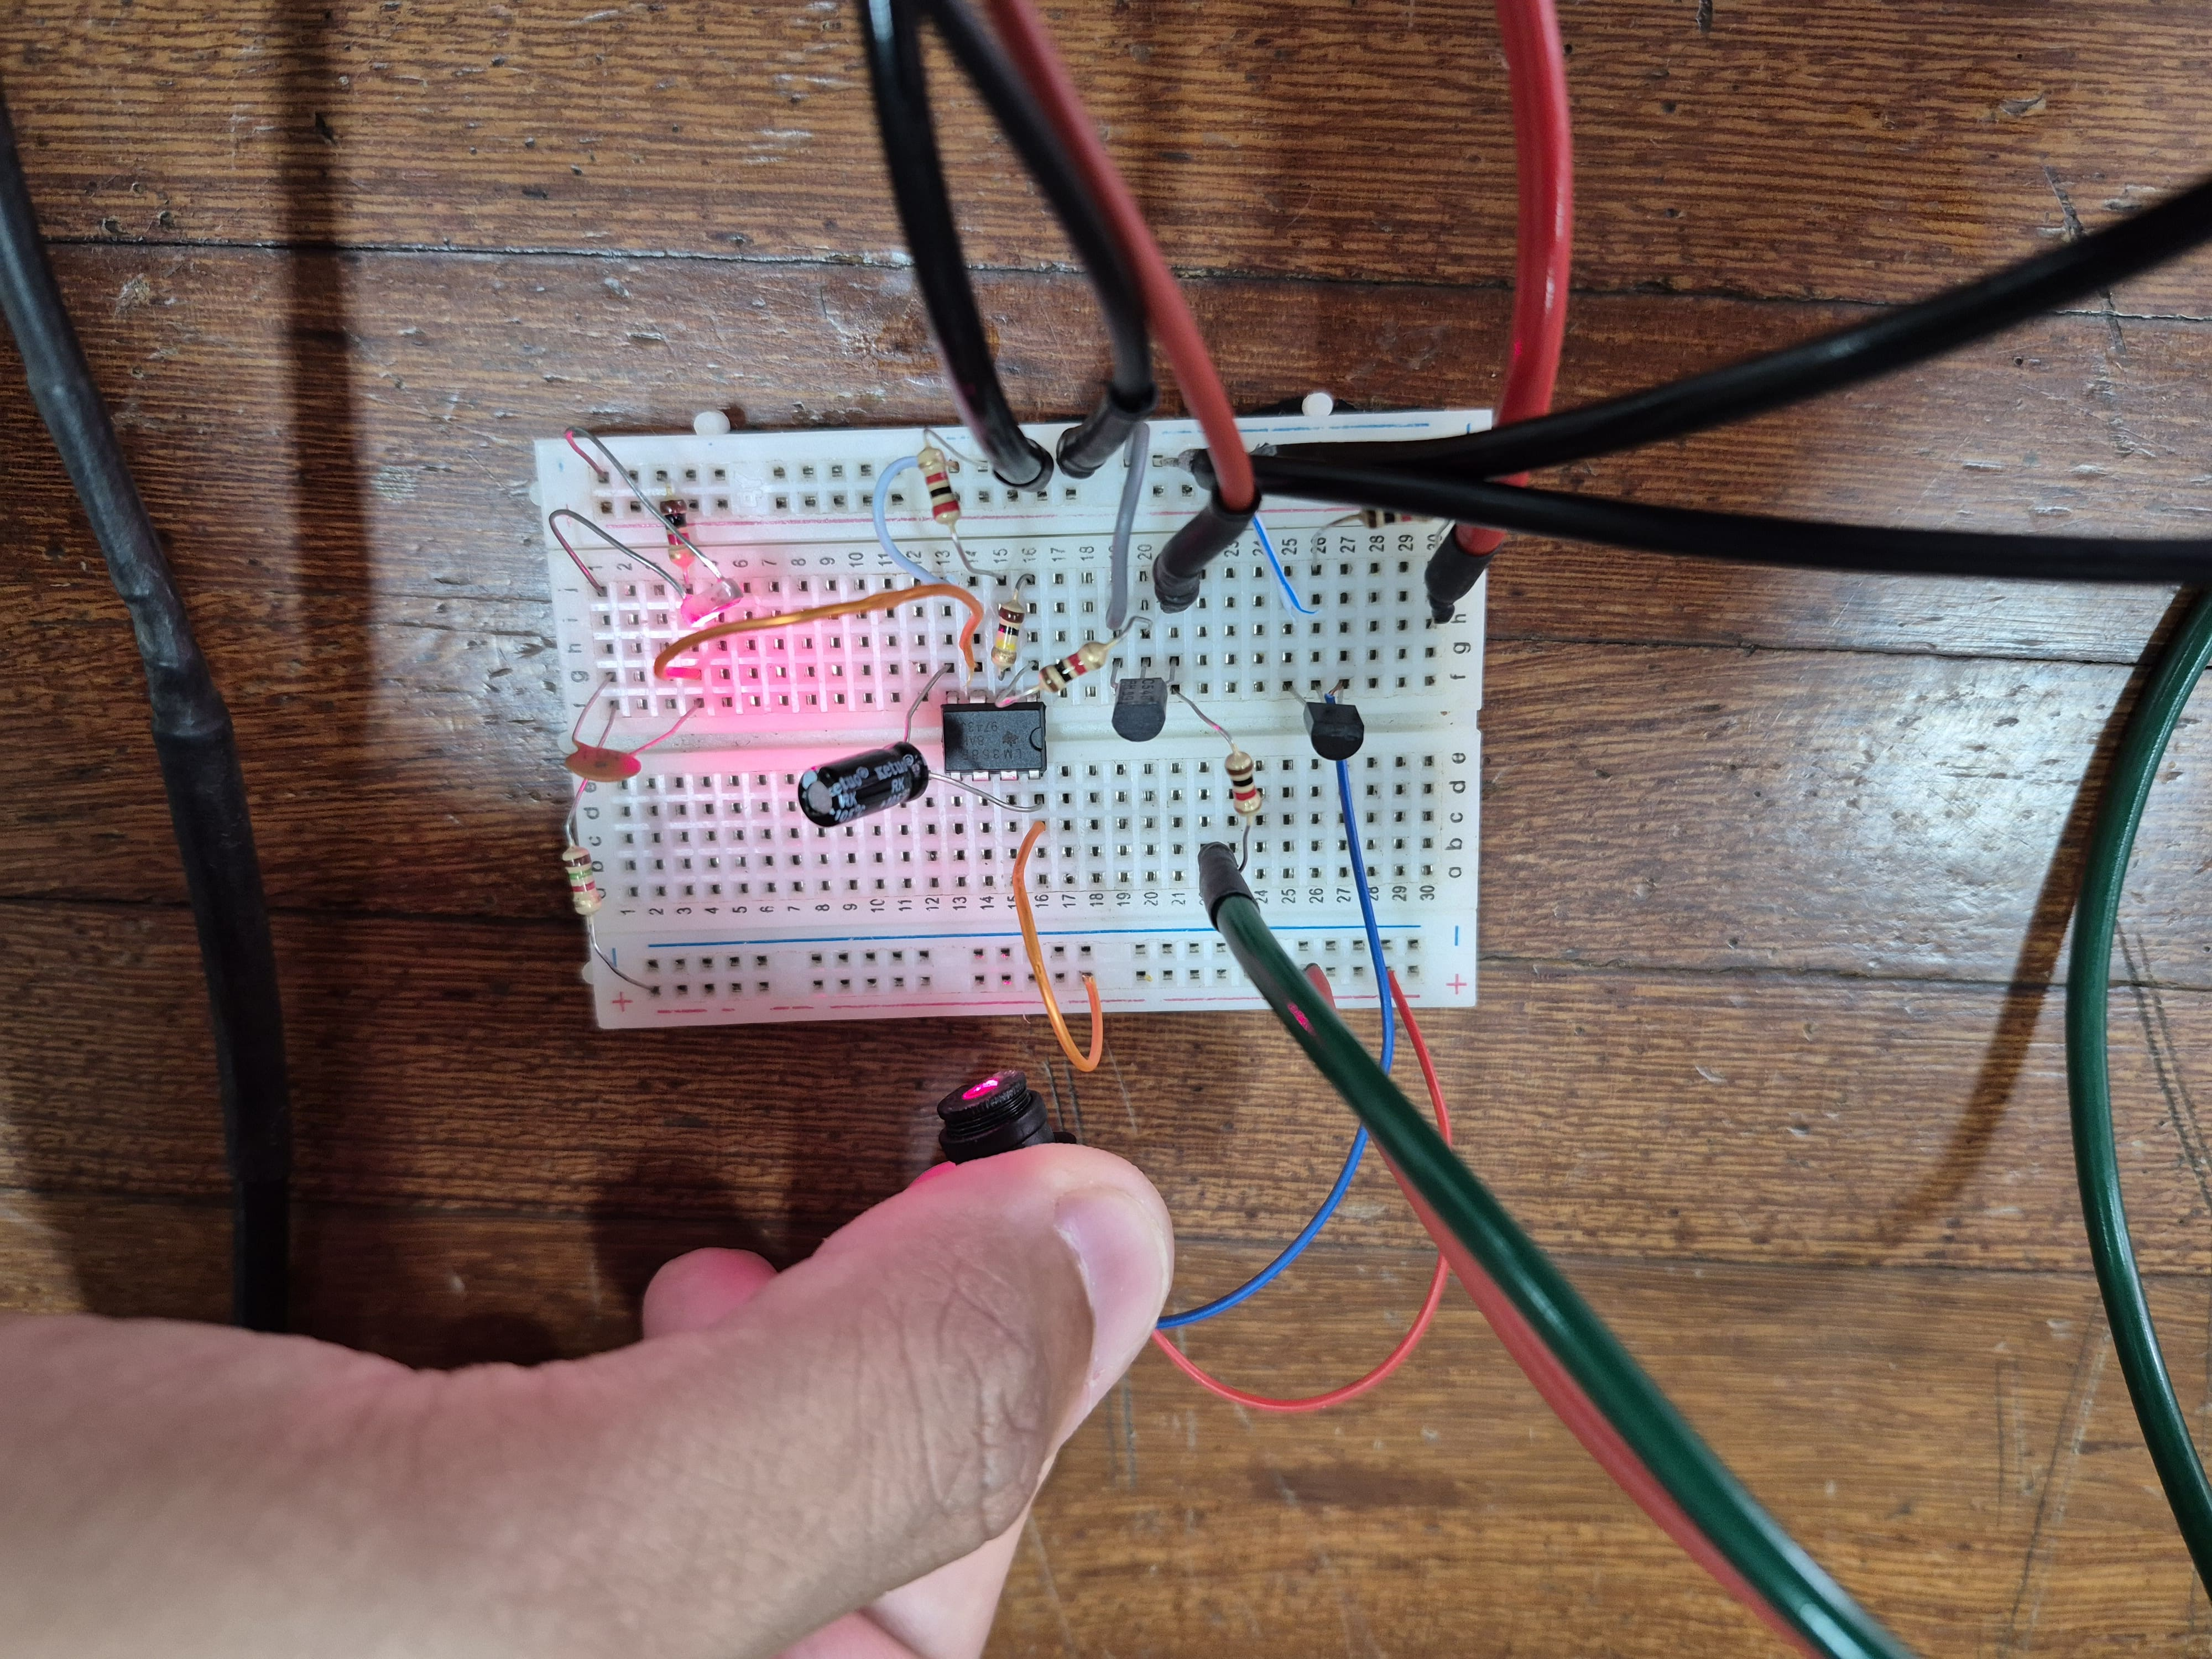
\includegraphics[width=0.5\linewidth]{figuras/Circuito_dos_lasers.jpg}
    \caption{Circuito dos lasers montado em bancada}
    \label{fig:circ_laser}
\end{figure}

\begin{figure}[H]
    \centering
    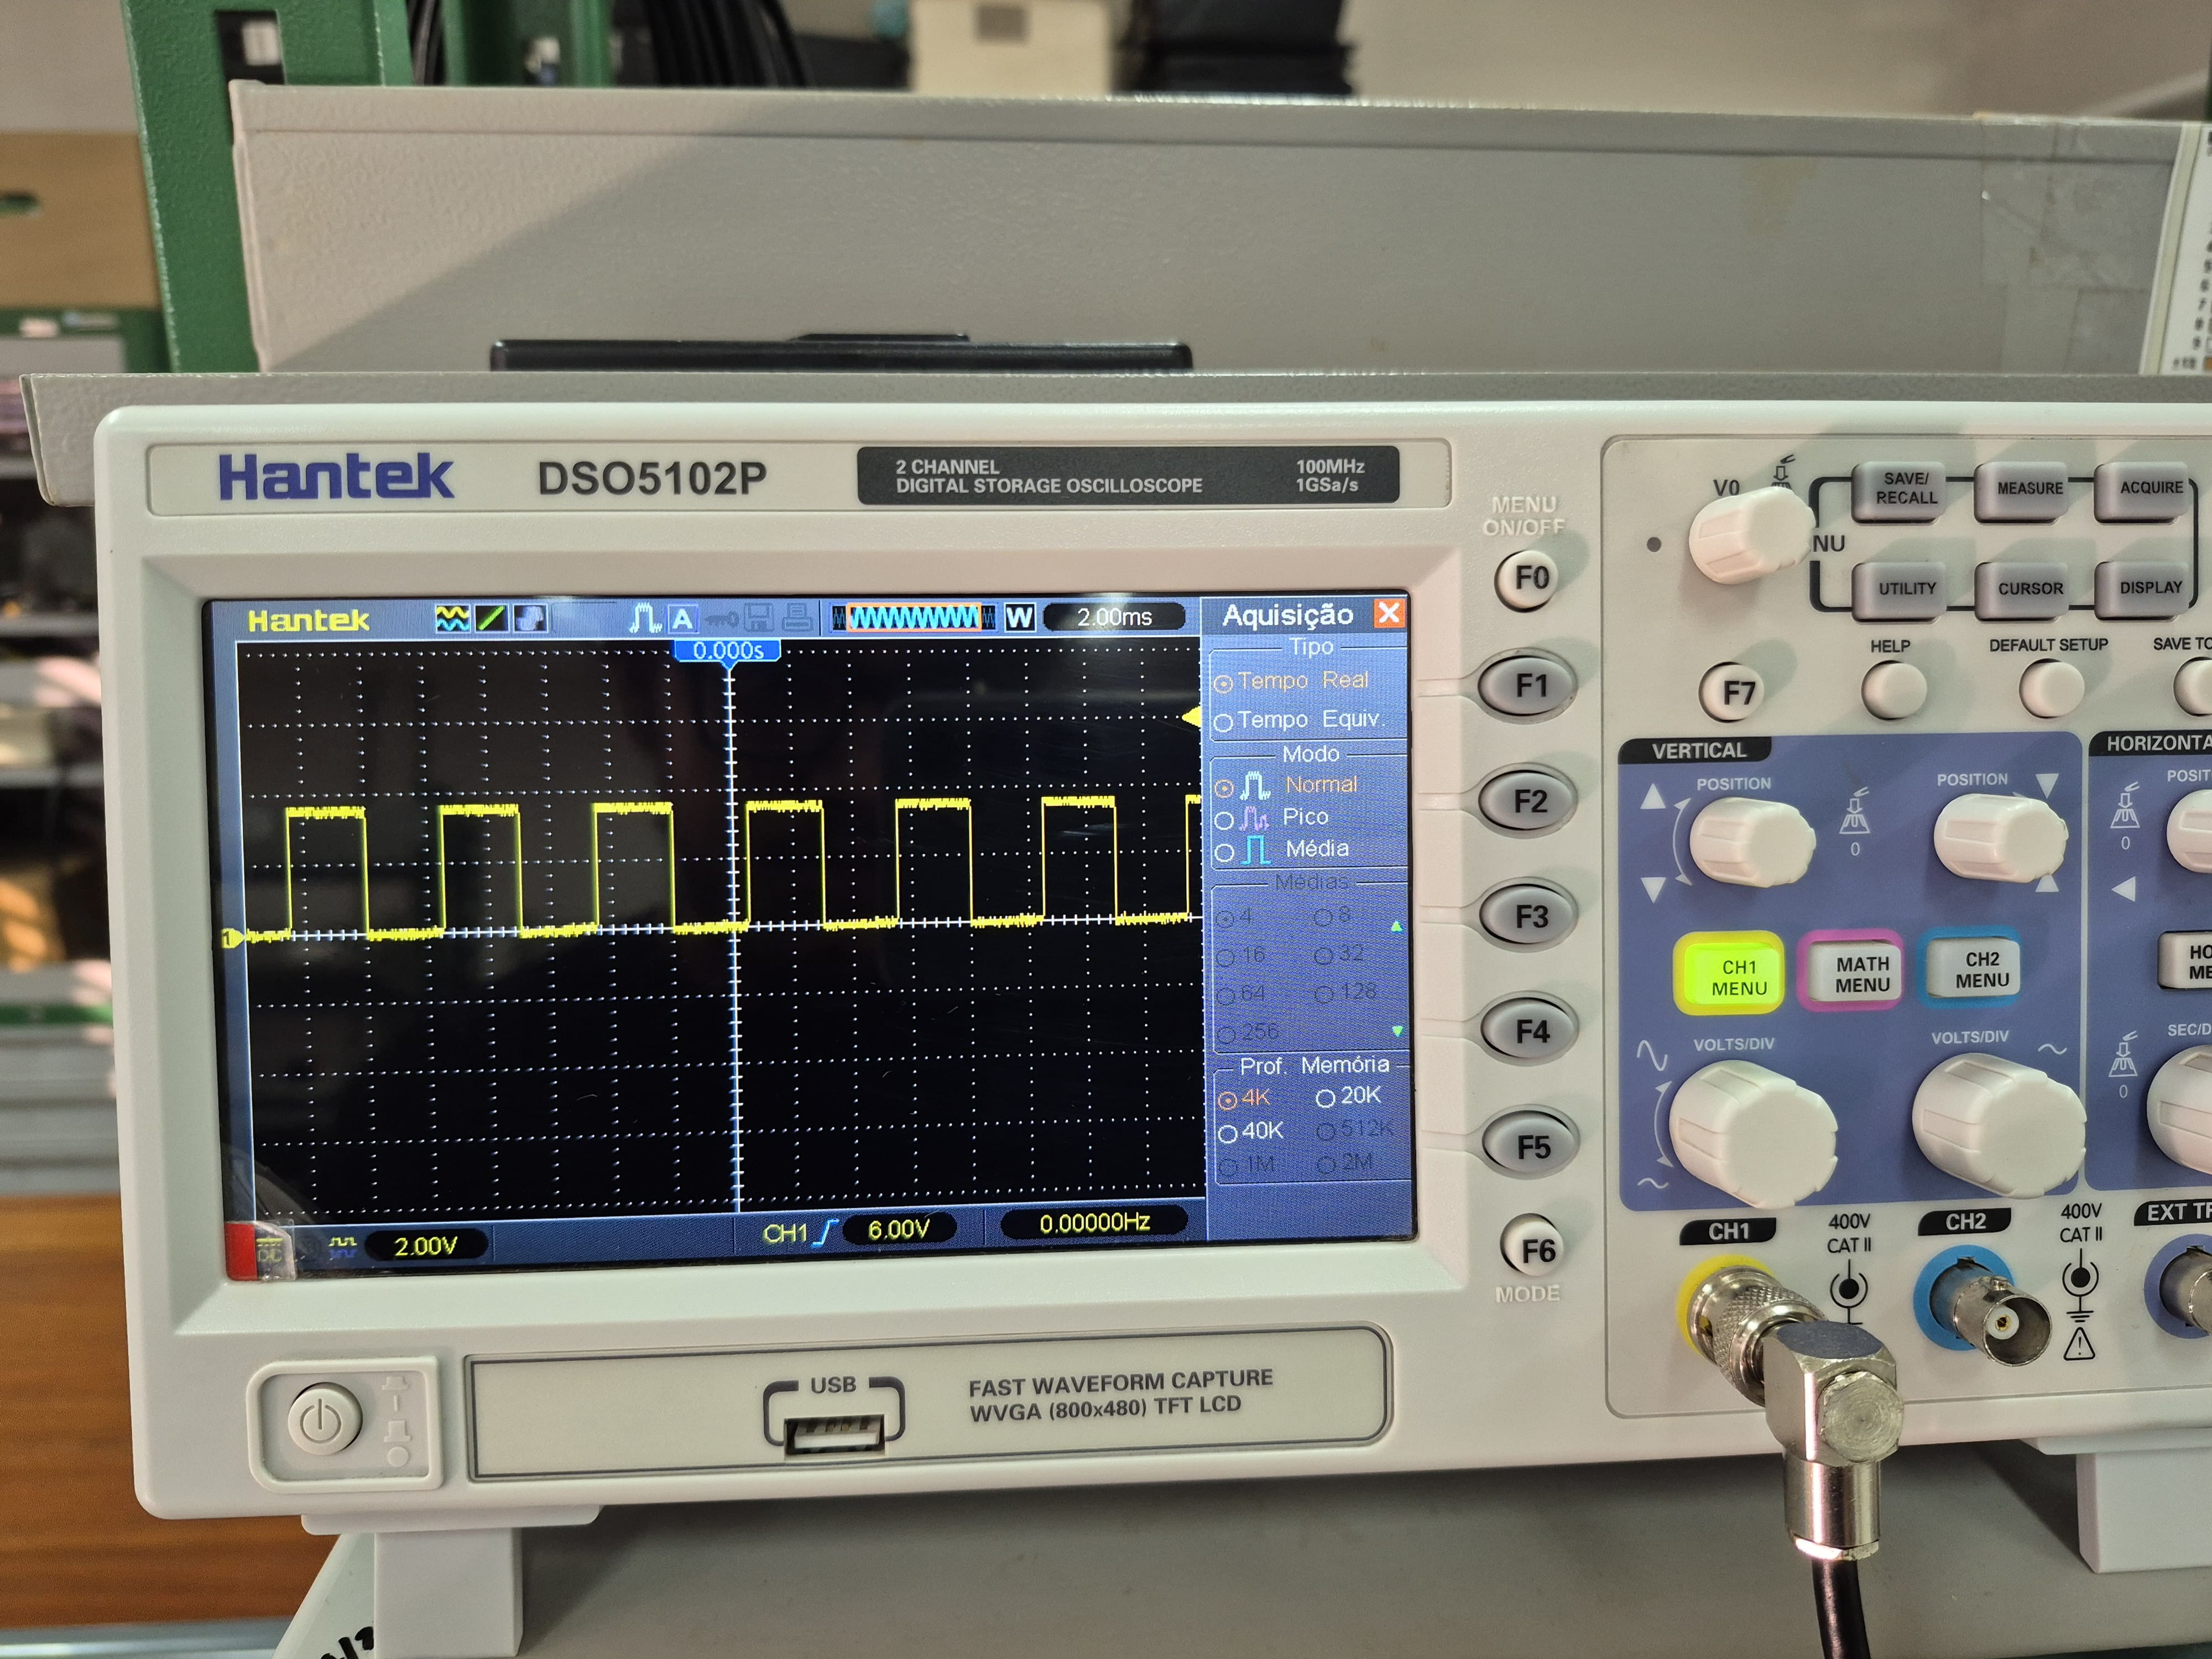
\includegraphics[width=0.5\linewidth]{figuras/Laser_sem_interrupcao.jpg}
    \caption{Laser sem interrupção}
    \label{fig:laser_sem_interrupção}
\end{figure}

\begin{figure}[H]
    \centering
    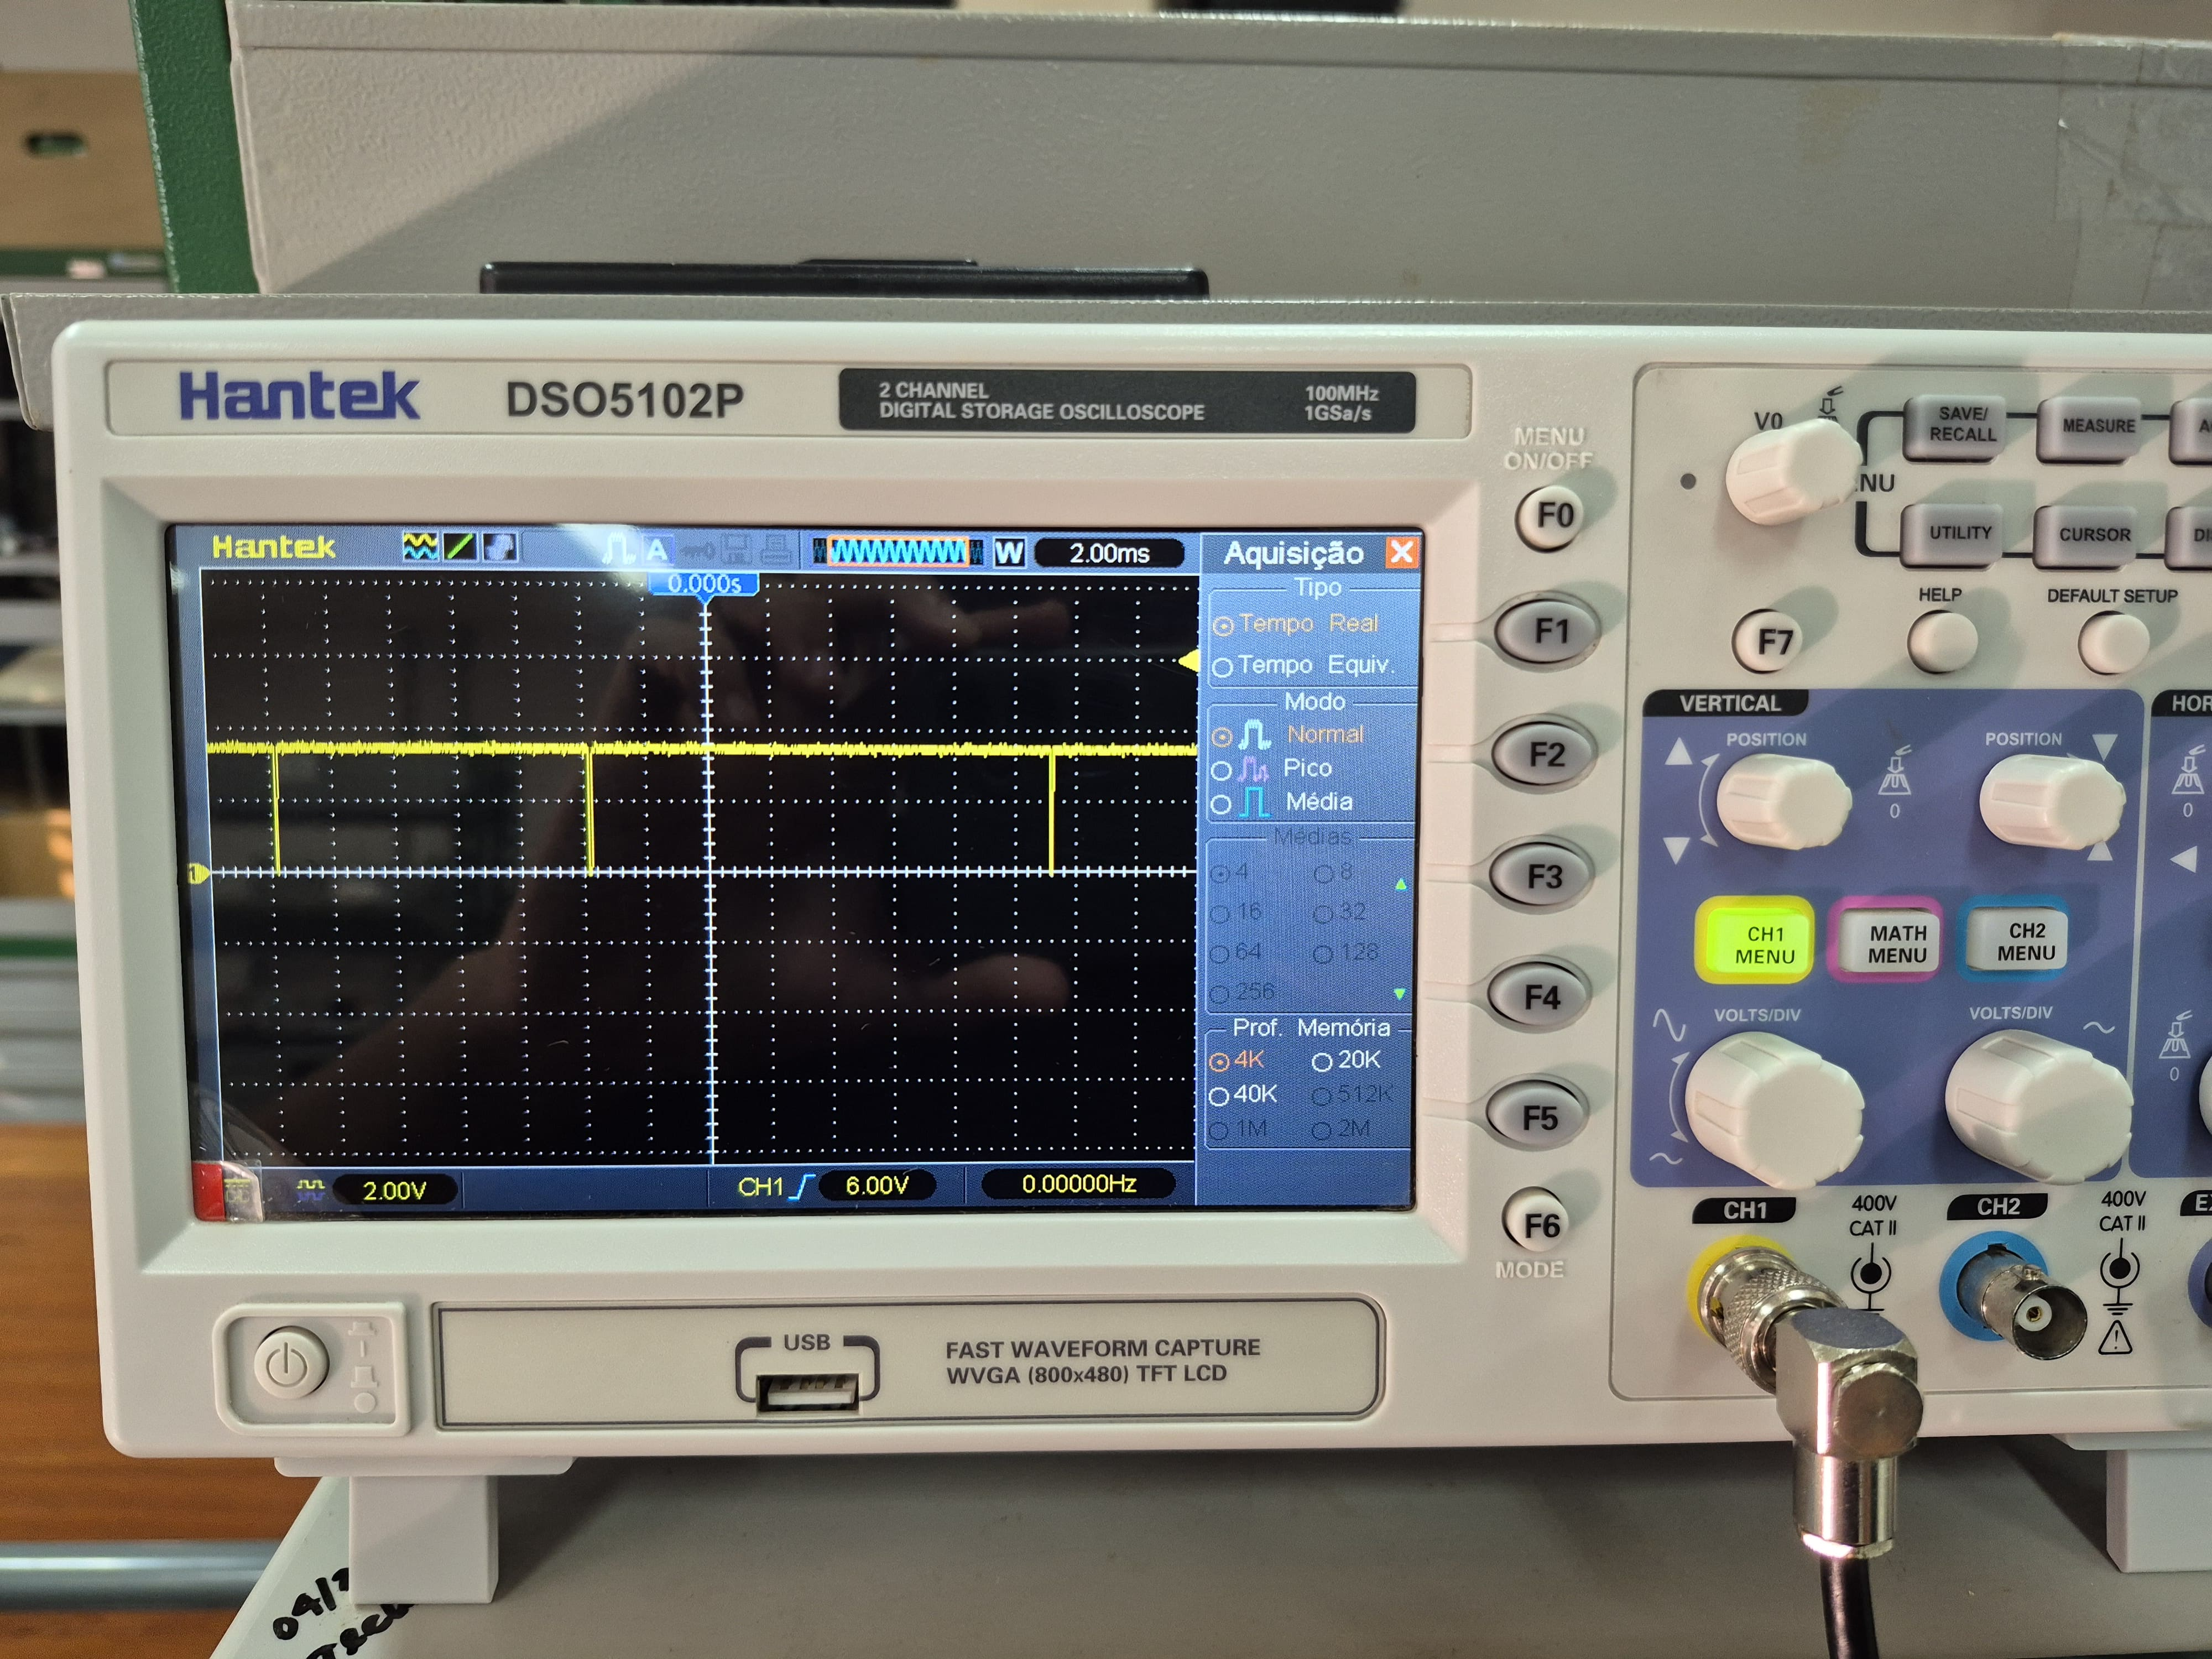
\includegraphics[width=0.5\linewidth]{figuras/Laser_interrompido.jpg}
    \caption{Laser interrompido}
    \label{fig:laser_interrompido}
\end{figure}

\paragraph{\textit{Flash} (luminária).}
O controle via PWM funciona corretamente, alterando a intensidade do brilho do \textit{flash} no modo FSM e ativando e desativado em resposta aos comandos assíncronos recebidos via UART, sem instabilidades observadas.

\paragraph{Motor de passo.}
O motor opera de forma estável em frequências mais baixas de acionamento. Os testes indicaram que o controle de velocidade por alteração do ARR do TIM6 funciona, porém com uma faixa operacional limitada --- comportamento esperado dadas as características físicas do motor de passo (torque \textit{versus} velocidade). Em razão disso, a velocidade de operação será mantida fixa no valor mínimo configurado (\texttt{STEPPER\_MIN\_VEL} $=$ 300\,passos/s), que corresponde a um período de interrupção do TIM6 de aproximadamente 1,67\,ms, calculado com base na configuração de \textit{prescaler} de 63 e \textit{clock} de 64\,MHz.

\paragraph{Servo motor.}
O servo motor ES08MA responde corretamente a qualquer valor de angulação dentro da faixa suportada (0° a 180°). Para a aplicação na esteira, os ângulos definidos no \textit{firmware} --- 0° para cancela fechada (Rota~A) e 45° para cancela aberta (Rota~B) --- foram validados e apresentaram o posicionamento mecânico desejado.

\paragraph{Dimensões do código QR.}
Observando o comportamento da câmera, foi possível verificar que um código QR com dimensões de 3×3\,cm conseguiu ser lido com maior facilidade do que um código QR com dimensões de 5×5\,cm. Além disso, para auxiliar na leitura do código, foi implementada uma rotina de \textit{fade-in/fade-out} do flash, garantindo que houvesse uma variação na luminosidade incidente no código QR. Essa variação auxiliou a leitura do código por permitir que o ajuste automático de saturação da \textit{webcam} se adaptasse à variação de luz ambiente, permitindo que ao menos um dos quadros capturados pelo sensor estivesse suficientemente nítido para a correta interpretação do código pelo algoritmo.

\paragraph{Instabilidades observadas na versão}

Durante o desenvolvimento e validação do sistema, foram identificadas instabilidades
que demandaram refinamentos ao longo do ciclo de implementação. No âmbito do
\textit{software}, três ocorrências foram tratadas: a interface de linha de comando
desenvolvida em C apresentava comportamento inconsistente em determinadas sequências
de operação, exigindo revisão da lógica de controle e do fluxo de execução; o
procedimento de \textit{reset} por software do STM32G070, acionado via comando
\texttt{SW\_RESET} pela interface, não respeitava o intervalo mínimo necessário para
a reinicialização completa do microcontrolador, causando falha no handshake subsequente;
por fim, foi identificada uma condição de corrida na etapa de inicialização do sistema,
em que o Raspberry Pi 3B tentava estabelecer comunicação antes que os periféricos do
STM32G070 estivessem devidamente configurados, resultando em perda do frame de
handshake.

Como perspectiva para o próximo ponto de controle, no âmbito do \textit{hardware}, prevê-se a
incorporação de um \textit{display} e de um botão físico à plataforma Raspberry Pi 3B.
Tais recursos permitiriam ao operador interagir diretamente com o sistema embarcado
sem depender de um terminal externo, tornando a operação mais autônoma e a interface
com o usuário mais intuitiva, características desejáveis para uma versão de produto
consolidada.


